\documentclass[12pt,a4paper]{article}
\usepackage[utf8]{inputenc}
\usepackage[spanish]{babel}
\usepackage{amsmath}
\usepackage{amsfonts}
\usepackage{amssymb}
\usepackage{makeidx}
\usepackage{graphicx}
\usepackage{multicol}
\usepackage{changepage}
\usepackage{float}
\usepackage{cite}
\usepackage{url}
\usepackage[left=2cm,right=2cm,top=2cm,bottom=2cm]{geometry}

\begin{document}
%encabezado 
\pagestyle{plain}{
\pagestyle{empty}
\changepage{3cm}{1cm}{-0.5cm}{-0.5cm}{}{-2cm}{}{}{}
\noindent
{
\small
\begin{tabular}{p{0.75\textwidth} p{0.25\textwidth} }

\includegraphics[scale=0.3]{logoUniversidad.png}&
\includegraphics[scale=0.5]{images.jpg} 
\end{tabular}
}
%datos de la caratula
\begin{center}
\par\vspace{2cm} %Rspacoo dejado antes del encabezado
{
\Huge\textbf{
Universidad de Guayaquil \\*[0.40cm] Facultad de Ciencias Matem\'aticas y F\'isicas}
}
\par\vspace{2cm}
{
\Large\textbf{Integrantes:}
\par\vspace{0.2cm}
\Large\textbf{Castro Alexander}\\
\Large\textbf{Chea M. Bethsaida} \\
\Large\textbf{Flores R. Emanuel}\\
\par\vspace{0.5cm}
\Large\textbf{Proyecto basado en la norma ISO 9001:20152}
\par\vspace{1cm}
\Large\textbf{Ingenier\'ia de Software}
\par\vspace{1cm}
\Large\textbf{Materia: Procesos de Software}
\par\vspace{1cm}
\Large\textbf{Docente: Ing. Miguel \'Angel Botto Tobar }
}
\par\vspace{2cm}
\large\textbf{ 5/03/2020}
\par\vspace{0.5cm}
\large\textbf{2019-2020} 
\par\vspace{3cm} 

\end{center}
\clearpage
}

\tableofcontents
\par\vspace{16cm}

\section{Norma ISO 9001}\textbf{}

ISO 9001 es la norma sobre gestión de la calidad con mayor reconocimeinto en todo el mundo. Pertenece a la familia ISO 9000 de normas de sistemas de gestión de la calidad (junto con ISO 9004), y ayuda a las organizaciones a cumplir con las expectativas y necesidades de sus clientes, entre otros beneficios.

Un sistema de gestión ISO 9001 le ayudará a gestionar y controlar de manera continua la calidad en todos los procesos. Como norma de gestión de la calidad de mayor reconocimiento en el mundo, así como el standard de referencia, describe cómo alcanzar un desempeño y servicio consistentes.

\section{Introducción}\textbf{}
PEÑACA es una empresa que distribuye y comercializa suministros de oficina, útiles escolares y toda gama amplia de papelerías a nivel nacional; así como también cuenta con una industria de conversiones de cartulinas y papeles para el sector gráfico.
Por esta razón se facilitará un software que ayude y optimice de manera indispensable el proceso de trabajo que realiza la empresa para así reducir el tiempo de procesamiento de información que una persona promedio puede llevar a cabo de manera manual en vez de una forma digital.
\begin{center}

\includegraphics[width=0.9\textwidth]{Peñaca.png}   
\end{center}

\vspace{8cm}
\section{Casos de estudio}\textbf{}
\begin{center}
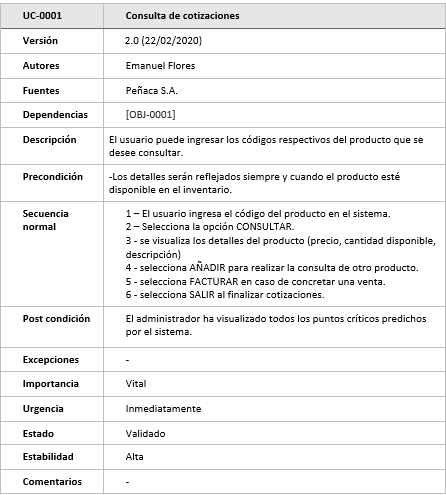
\includegraphics[width=0.9\textwidth]{casodeusouno.png}   
\end{center}
\begin{center}
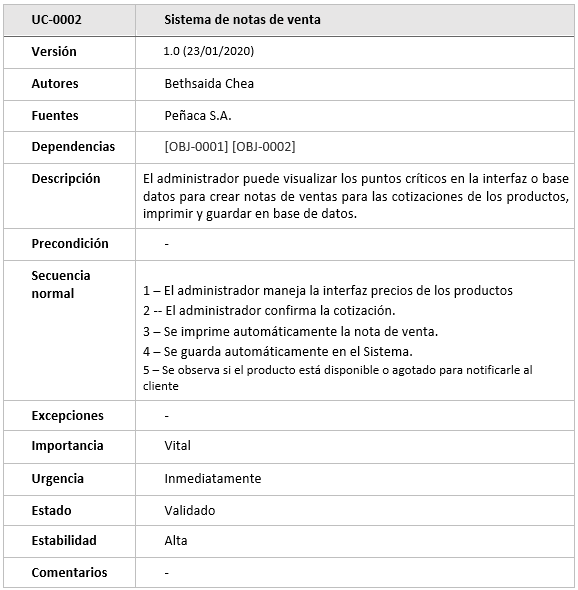
\includegraphics[width=0.9\textwidth]{casodeusodos.png}   
\end{center}


\section{Sistema de gestión de calidad}\textbf{}
\subsection{Requisitos Funcionales}
1.	Crear facturas en el momento de vender el producto, imprimir y guardar en base de datos.\\\\
Descripción: En el área de ventas, al realizar la venta de un producto de la empresa que si se encuentra en el inventario y consta en los registros, se generará una factura la cual automáticamente se imprimirá al confirmar la venta y además esta se guardará en una base de datos para tener una constancia digital.
En caso de que el producto solicitado se haya agotado se dará la opción de modificar el pedido o cancelarlo. 
\\\\
2.	Crear notas de ventas para las cotizaciones de los productos, mostra y guardar en el sistema.\\\\
Descripcion:En el área de ventas, al realizar una cotización de precios de productos de la empresa se generará nota de ventas la cual automáticamente se imprimirá al confirmar que dicha cotización concluyó, además esta se guardará en una base de datos para tener una constancia digital.
También se podrá observar si el producto está disponible o si está agotado para así poder notificarle al cliente.
\\\\
3.	Registrar datos de clientes nuevos en el sistema.\\\\
Descripción: Al realizar una venta se procederá a solicitar los datos del cliente los cuales son importantes para cualquier inconveniente con el producto y a su vez esta información se guardará en una base de datos y un fichero del cliente será creado para todas las facturas del cliente.
\\\\
4.	Comprobar datos de clientes en el sistema y modificarlos de ser solicitado.\\\\
Descripción: Comprobar si el cliente existe en el sistema para así optimizar tiempo en la recolección de datos fundamentales al realizar una factura, además se podrá modificar cualquier información en caso de que el cliente desee actualizarla.
\\\\
5.	Registrar mercadería nueva y realizar un conteo de los productos.\\\\
Descripción: En el área de inventario, se  realizará un registro de la mercadería nueva ingresada, además llevará un conteo de los productos disponibles en bodega.
En caso que se realizará una venta, el conteo del inventario se realizará nuevamente y la información estará actualizada.
\\\\
6. Obtener  precios  del proveedor\\\\
Descripción: El sistema llevará el registro de los diferentes proveedores de la empresa, en este se podrá seleccionar la cantidad de productos a adquirir  y el precio unitario y total por producto.

\subsection{Requisitos No Funcionales}

1.	El sistema contará con interfaces gráficas bien formadas.\\\\
Descripción: El diseño arquitectónico visible en el sistema será lo más Entendible para los usuarios de forma que  no se tengan complicaciones o dudas con respecto al manejo del sistema.
\\\\
2.	Diseño visual con  un entorno agradable para los usuarios.\\\\
Descripción: Contendrá iconos amigables y minimalista que hagan un buen contraste con el diseño de cada  ventana, para que sea más intuitivo y estético
\\\\
3.	Diseño que ayude a reconocer que se han llenado todos los datos para el registro.\\\\
Descripción: Contendrá una sub-ventana donde se registren los nuevos usuarios y señalará los campos que son obligatorios llenar para poder registrarse y notificara si al momento de registrarse no se han llenado dichos campos
\\\\


\section{Referencias normativas}\textbf{}
ISO 9001: 2015, Sistemas de gestión de calidad. Fundamentos y vocabulario.



\section{Contexto de la organización}\textbf{}
El contexto de la empresa PEÑACA S.A. consiste en distribuir cartulinas, papeles y suministros gráficos, los cuales son importados y otros fabricados por si mismos mediante la convertidora “PEÑAPAPEL”, para la industria Gráfica y labores Artesanal, ofreciendo servicio de corte desde A0 hasta A6, desarrollando procesos con eficiencia y eficacia.
 
\subsection{Dominio}
El dominio de la empresa PEÑACA S.A. se enfoca en la importación de cartulinas de distintos tipos y gramajes del mercado, brindando un servicio de calidad con la finalidad de entrega inmediata y la variedad, y ofrecer a sus clientes un precio conveniente al por menor y mayor para pequeñas y grandes industrias del país.

\subsection{Procesos}
Procesos de Ventas.

Area de Vendedores:
\begin{itemize}
\item Realiza cotizaciones de facturas.
\item Transmite la información de las cotizaciones a facturación.
\item Realiza notas de pedido a proveedores.
\item Confirmación de mercaderías que han sido retiradas o enviadas.\\\\
\end{itemize}

Area de Facturación:
\begin{itemize}
\item Registra los datos de nuevos clientes en la empresa.
\item Recibe la información de la cotización realizada en el área de ventas.
\item Se crea la factura en base a la cotización.\\\\
\end{itemize}

Area de Inventario:
\begin{itemize}
\item Registra la mercadería comprada.
\item Lleva control de la mercadería vendida.
\item Proporciona mercadería para la venta.\\\\
\end{itemize}

Area de Compras:
\begin{itemize}
\item Consulta precio del proveedor.
\item Adquiere mercadería.
\item Verifica inventario.\\\\
\end{itemize}

\subsection{Políticas}
\textbf{Comunicación de la política de calidad}\\\\
La información del programa está disponible en la página de la empresa y cuenta con los manuales necesarios para la utilización de este.
El programa también cuenta con dos versiones de pago, las cuales dan acceso a llamadas telefónicas para servicio al cliente mientras que la versión básica, es decir la gratuita cuenta con servicio al cliente por vía mensajería; manteniendo así contacto la empresa desarrolladora del producto y el cliente.


\section{Planificación}\textbf{}
Al realizar el SGC, la empresa consideró varios puntos importantes, como lo son el alcance, los procesos y los requerimientos referidos, para así determinar los riesgos y oportunidades que se van a abordar con la finalidad de:
\begin{itemize}
\item Asegurar que se cumplan los resultados
\item Aumentar los efectos deseables
\item Prevenir o reducir los efectos no deseados
\item Lograr mejoras
\end{itemize}
Las acciones tomadas para abordar los riesgos y oportunidades son proporcionales al impacto potencial en la conformidad del producto que brinda la empresa.
\vspace{17cm}

\subsection{Diseño del producto}
\par\vspace{0.5cm}
\textbf {Inicio del Programa de Peñaca}\\\\
\begin{center}
\includegraphics[scale=0.7]{inicio.png}
\end{center}
\par\vspace{1cm}
\textbf {Registro}\\\\
\begin{center}
 \includegraphics[scale=0.7]{registro.png}
 \end{center} 
 \par\vspace{0.5cm}
\textbf {Nuevo Cliente}\\\\
\begin{center}
 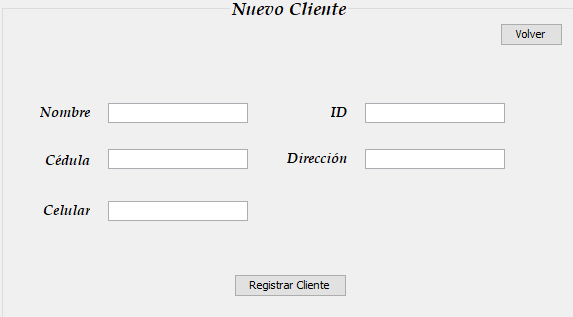
\includegraphics[scale=0.7]{nuevocliente.png} 
 \end{center}
 \par\vspace{2cm}
\textbf {Inventario}\\\\
\begin{center}
 \includegraphics[scale=0.7]{inventario.png} 
 \end{center}
 \par\vspace{0.5cm}
\textbf {Registrar Proveedor}\\\\
\begin{center}
 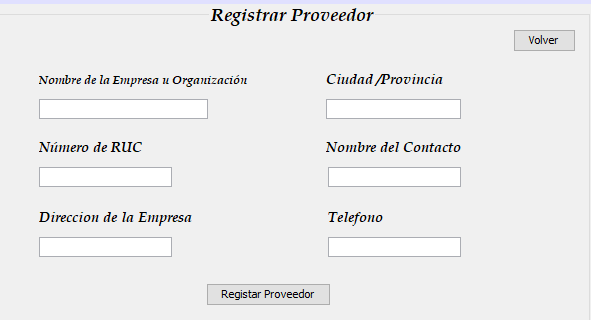
\includegraphics[scale=0.7]{registroprove.png} 
 \end{center}
 \par\vspace{2cm}
\textbf {Facturas}\\\\
\begin{center}
 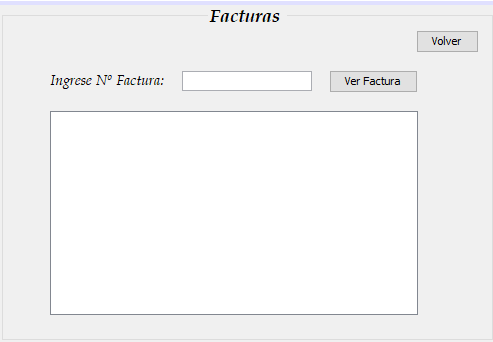
\includegraphics[scale=0.7]{Facturas.png} 
 \end{center}

\section{Conclusiones}\textbf{}
Una vez ya informados de los procesos que realizar a diario se reconocemos los requerimientos que se implementan para automatizar y logramos respuestas inmediatas.

Indagando cuál es su dominio y funciones, elaboramos los requisitos funcionales que desarrollamos dentro del sistema cumpliendo los requerimientos encontrados en el OBJ-0001

Representando los diagramas de flujo, se organiza qué procesos se irán realizando según la secuencia en el desarrollo. 

Conociendo qué actores intervienen, logramos asignar funciones dentro del sistema para cada usuario, un ejemplo sería que la persona que compra los materiales no puede ingresar en el área de ventas por que no sabría a qué porcentaje se vende los productos y podría causar pérdida a la empresa. Por eso cada usuario maneja su área sin acceso a otra que no le corresponde.  

 \par\vspace{6cm}\section{Referencia}\textbf{}
https://github.com/Stefan-Castro/ProyectoProcesosSecondP
\end{document}
